\setcounter{ex}{0}
\section{HÀM SỐ MŨ- HÀM SỐ LOGARIT}
\subsection{Bài tập rèn luyện}
\Opensolutionfile{ans}[ans/DA-CD6-MU-LOGARIT-VD]
\begin{ex}%[2D2Y1-1]%[An Do]
Cho $a$ là một số thực dương, biểu thức $\sqrt[3]{\dfrac{1}{a}}$ bằng
\choice{$a^3$}{$a^{\tfrac{1}{3}}$}{\True$a^{\tfrac{-1}{3}}$}{$a^{\tfrac{1}{2}}$}
    \loigiai{
        $\sqrt[3]{\dfrac{1}{a}} = \sqrt[3]{a^{-1}} = a^{-\tfrac{1}{3}}$, với $a>0$.
    }
%\dotlineEX{1}
\end{ex}
\begin{ex}[Phan Bội Châu Nghệ An 2025 - Lần 1] Cho các số thực dương $a, b$ với $a \neq 1$ thỏa mãn $\log_a b = 5$. Giá trị của biểu thức $\log_a (ab)$ bằng
\choice
{7}
{4}
{5}
{\True $6$}
\loigiai{
    
}
\end{ex}
\begin{ex}[KHTN HN 2025 - Lần 2]
Biết $a, b$ là các số thực dương, khác 1 thỏa mãn $\log_a b = 3$. Giá trị của biểu thức $\log_a \frac{a}{\sqrt{b}}$ bằng
\choice
{$\frac{5}{8}$}
{$\frac{5}{2}$}
{\True $-\frac{1}{4}$}
{$\frac{3}{2}$}
\loigiai{
    
}
\end{ex}
\begin{ex}[SGD Hưng Yên-Lần 1-2026] % Câu 11
Cho $\log_a b = 5$. Giá trị của biểu thức $\log_a\left(a^2 b\right)$ bằng:
\choice
{\True $7$}
{$20$}
{$25$}
{$10$}
\loigiai{
    Ta có: $\log_a\left(a^2 b\right) = \log_a \left(a^2\right) + \log_a b = 2 + 5 = 7$.
}
%\dotlineEX{1}% Tạo các dòng kẻ trong tài liệu
\end{ex}
\begin{ex}%[2D2Y4-1]%Câu 5
Tập xác định của hàm số $y=\log_3 \left(2x+1\right)$ là
\choice
{$\left(-\infty;\dfrac{1}{2}\right)$}
{ $\left(\dfrac{1}{2};+\infty\right)$}
{$\left(0;+\infty\right)$}
{\True $\left(-\dfrac{1}{2};+\infty\right)$}
%\loigiai
%{
%    Hàm số $y=\log_3 \left(2x+1\right)$ xác định khi và chỉ khi $2x+1>0 \Leftrightarrow x>-\dfrac{1}{2}$.\\
%    Vậy tập xác định của hàm số là $\mathscr{D} = \left(-\dfrac{1}{2};+\infty\right)$.
%}
\dotlineEX{2}
\end{ex}
\begin{ex}%[2D2Y2-1]%Câu 1
Tập xác định của hàm số $y=\left(3-x\right)^\frac{2}{3}$ là 
\choice
{\True $\left(-\infty;3\right)$}
{$\left(-\infty;-3\right)$}
{$\left(3;+\infty\right)$}
{$\left(-\infty;+\infty\right)$}
\loigiai
{
    Hàm số $y=\left(3-x\right)^\frac{2}{3}$ xác định khi và chỉ khi $3-x>0 \Leftrightarrow x<3$.\\
    Vậy tập xác định của hàm số là $\mathscr{D} = \left(-\infty;3\right)$.
}
\end{ex}
\begin{ex}%[Lê Thị Thanh Tuyền-DA1]%[2D2B4-3]
\immini[thm]{
    Đường cong trong hình bên là đồ thị của hàm số nào.
    \choice
    {$y=\left(\dfrac{1}{2}\right)^x$}
    {$y=\log_{\frac{2}{5}} x$}
    {$y=\log_3 x$}
    {\True $y=2^x$}
}{
    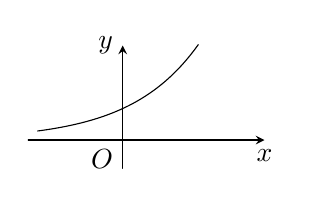
\begin{tikzpicture}[>=stealth, line join=round, line cap=round,x=.6cm,y=.4cm]
        \def\xmin{-2} \def\xmax{3} \def\ymax{3}
        \draw[->] (\xmin,0)--(\xmax,0) node [below]{$x$};
        \draw[->] (0,-0.9)--(0,\ymax) node [left]{$y$};
        \node at (0,0) [below left]{$O$};
        \draw[smooth,samples=300,domain=-1.8:1.6] plot(\x,{2^(\x)});
    \end{tikzpicture}
}
\loigiai{
    Quan sát hình dáng đồ thị ta thấy đồ thị nằm trên trục $Ox$, đồ thị đi lên từ trái sang phải.
}
\end{ex}
\begin{ex}%[Lê Thị Thanh Tuyền-DA1]%[2D2B4-3]
\immini[thm]
{
    Cho hai hàm số $y=a^x$ và $y=\log_b x$ có đồ thị như hình vẽ. Mệnh đề nào sau đây là đúng.
    \choice
    {\True $a>1; 0<b<1$}
    {$0<a<1; 0<b<1$}
    {$0<a<1; b>1$}
    {$a>1; b>1$}
}
{
    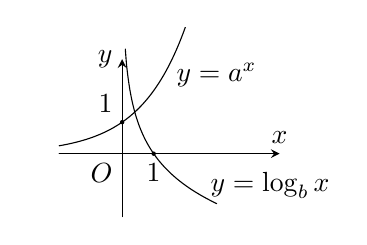
\begin{tikzpicture}[>=stealth,scale=.4, line join=round, line cap=round]
        \draw[->] (-2,0)--(5,0) node [above]{$x$};
        \draw[->] (0,-2)--(0,3) node [left]{$y$};
        \node at (0,0) [below left]{$O$};
        \node at (3,2.5){$y=a^x$};
        \node at (2.5,-1)[right]{$y=\log_{b}x$};
        \clip (-3,-2) rectangle (6,4);
        \fill[black](0,1) circle (2pt) node[above left] {$1$} (1,0) circle (2pt) node [below] {$1$};
        \draw[smooth,samples=150,domain=-2:3] plot(\x,{2^(\x)});
        \draw[smooth,samples=150,domain=0.1:3] plot(\x,{-ln(\x)/ln(2)});
        
    \end{tikzpicture}
}
\loigiai{
    Quan sát đồ thị ta thấy :\\
    Đồ thị hàm số $y=a^x$ đi lên từ trái sang phải nên hàm số đồng biến, tức $a>1$.\\
    Đồ thị hàm số $y=\log_b x$ đi xuống từ trái sang phải nên hàm số nghịch biến, suy ra $0<b<1$.
}
\end{ex}
\begin{ex}[Sở Ninh Bình 2025 - Lần 2]
Nghiệm của phương trình $5^x = 3$ là
\choice
{$\sqrt[5]{3}$}
{$\sqrt[3]{5}$}
{\True $\log_5 3$}
{$\log_3 5$}
\loigiai{
    
}
\end{ex}
\begin{ex}
Nghiệm của phương trình $\log_2(x-1)=3$ thuộc khoảng nào dưới đây?
\choice
{$(6; 8)$}
{\True $(8; 10)$}
{$(3; 5)$}
{$(10; 12)$}
\loigiai{
    Điều kiện xác định: $x-1>0 \Leftrightarrow x>1$.
    Ta có phương trình:
    $$\log_2(x-1)=3 \Leftrightarrow x-1=2^3 \Leftrightarrow x-1=8 \Leftrightarrow x=9 \text{ (thỏa mãn).}$$
    Vì $9 \in (8; 10)$ nên nghiệm của phương trình thuộc khoảng $(8; 10)$.
}
\end{ex}
\begin{ex}[ĐH Vinh 2025 - Lần 1]
Tập nghiệm của bất phương trình $3^{3x + 1} < \frac{1}{9}$ là
\choice
{$(-1; +\infty)$}
{$(-\infty; 1)$}
{$(1; +\infty)$}
{\True $(-\infty; -1)$}
\loigiai{
    
}
\end{ex}
\begin{ex}[Đề minh hoạ 2025]
Tập nghiệm của bất phương trình $\log_2 (x - 1) < 3$ là
\choice
{$(1; 9$)}
{$(-\infty; 9)$}
{$(9; +\infty)$}
{\True $(1; 9)$}
\loigiai{
    
}
\end{ex}
\begin{ex}[Phan Bội Châu lần 2-Nghệ An-2026] % Câu 4
Tập nghiệm của  $\log_{\frac{1}{2}}(2x-5) \ge 1$ là
\choice
{$\left(\frac{5}{2}; \frac{11}{4}\right)$}
{\True $\left(\frac{5}{2}; \frac{11}{4}\right]$}
{$\left(\frac{11}{4}; +\infty\right)$}
{$\left[\frac{11}{4}; +\infty\right)$}
\loigiai{
    Điều kiện: $2x - 5 > 0 \Leftrightarrow x > \frac{5}{2}$.
    Bất phương trình đã cho tương đương với:
    $$2x - 5 \le \left(\frac{1}{2}\right)^1 \Leftrightarrow 2x \le \frac{11}{2} \Leftrightarrow x \le \frac{11}{4}.$$
    Kết hợp với điều kiện, ta được tập nghiệm của bất phương trình là $S = \left(\frac{5}{2}; \frac{11}{4}\right]$.
}
\end{ex}
\begin{ex} % Câu 7
Cho ba số $a,b,c$ khác $0$ thoả mãn $4^a = 3^b = 6^c$. Tính giá trị của biểu thức $\frac{c}{a} + \frac{2c}{b}$.
\choice
{$3$}
{$0$}
{$1$}
{\True $2$}
\loigiai{
    Từ giả thiết $4^a = 3^b = 6^c$, suy ra:
    $$\heva{& 4 = 6^{\frac{c}{a}} \\ & 3 = 6^{\frac{c}{b}} \Rightarrow 3^2 = \left(6^{\frac{c}{b}}\right)^2 \Rightarrow 9 = 6^{\frac{2c}{b}}}$$
    Nhân vế theo vế hai đẳng thức trên, ta được:
    $$4 \cdot 9 = 6^{\frac{c}{a}} \cdot 6^{\frac{2c}{b}} \Leftrightarrow 36 = 6^{\frac{c}{a} + \frac{2c}{b}} \Leftrightarrow 6^2 = 6^{\frac{c}{a} + \frac{2c}{b}} \Leftrightarrow \frac{c}{a} + \frac{2c}{b} = 2.$$
}
\dotlineEX{3}
\end{ex}
\Closesolutionfile{ans}
% \subsection{BÀI TẬP RÈN LUYỆN}
\Opensolutionfile{ans}[ans/DA-CD6-MU-LOGARIT-BTRL]
\begin{ex}%[2D2Y1-1]%[An Do]
Với $a>0$ thì $P = a^{\tfrac{3}{2}} \cdot \sqrt[3]{a}$ bằng
\choice{$a^{\tfrac{1}{2}}$}{$a^{\tfrac{9}{2}}$}{\True$a^{\tfrac{11}{6}}$}{$a^3$}
%    \loigiai{
%        $P = a^{\tfrac{3}{2}} \cdot \sqrt[3]{a} = a^{\tfrac{3}{2}} \cdot a^{\tfrac{1}{3}} = a^{\tfrac{11}{6}}$, với $a>0$
%    }
\end{ex}
\begin{ex}%[2D2Y1-1]%[An Do]
Rút gọn biểu thức $Q = (\sqrt[5]{a})^3 : \sqrt{a\sqrt{a}}$ với $a>0$ ta được
\choice{$Q = a^{\frac{3}{20}}$}{$Q = a^{\frac{27}{20}}$}{$Q = a^{\frac{4}{5}}$}{\True$Q = a^{-\frac{3}{20}}$}
    \loigiai{
            Ta có $Q = (\sqrt[5]{a})^3 : \sqrt{a\sqrt{a}} = a^{\frac{3}{5}} : \sqrt{a \cdot a^{\frac{1}{2}}} = a^{\frac{3}{5}} : \sqrt{a^{\frac{3}{2}}} = a^{\frac{3}{5}} : a^{\frac{3}{4}} = a^{\frac{3}{5} - \frac{3}{4}} = a^{-\frac{3}{20}}$ với $a>0$.
        }
\end{ex}
\begin{ex}%[2D2B3-2]%[Thái Văn Đạt, tổng ôn MarieCurie]
Nếu $\log_a b = 2$ thì $\log_{a^4} \left(b^8 a^2\right)$ bằng
\choice
{\True $\dfrac{9}{2}$}
{$9$}
{$2$}
{$8$}
\loigiai{
    Ta có $\log_{a^4} \left(b^8 a^2\right) = \log_{a^4} b^8 + \log_{a^4} a^2 = \dfrac{8}{4}\log_a b + \dfrac{2}{4} \log_a a = 4 + \dfrac{1}{2} = \dfrac{9}{2}$.
}
\end{ex}
\begin{ex}%[2D2K3-1]%[Thái Văn Đạt, tổng ôn MarieCurie]
Cho $\log_a x = 3$, $\log_b x = 4$ với $a$, $b$ là các số thực lớn hơn $1$, khi đó $\log_{ab} x$ bằng
\choice
{$\dfrac{7}{12}$}
{$\dfrac{1}{12}$}
{$12$}
{\True $\dfrac{12}{7}$}
\loigiai{
    Ta có $\log_a x = 3$ và $\log_b x = 4$ nên $x = a^3 = b^4$ hay $a=x^{\frac{1}{3}}$ và $b=x^{\frac{1}{4}}$.\\
    Do đó $ab = x^{\frac{1}{3}+\frac{1}{4}} = x^{\frac{7}{12}}$.\\
    Vậy $\log_{ab} x = \log_{x^{\frac{7}{12}}} x = \dfrac{12}{7}\log_x x =\dfrac{12}{7}$.
}
\end{ex}
%Câu 25
\begin{ex}%[2D2B3-2]%[Thái Văn Đạt, tổng ôn MarieCurie]
Cho $\log_a b =2 $ và $\log_a c = 3$, khi đó $\log_a \left( b^2c^3 \right)$ bằng
\choice
{$31$}
{\True $13$}
{$30$}
{$108$}
\loigiai{
    Ta có $\log_a \left( b^2c^3 \right) = \log_a b^2 + \log_a c^3 = 2\log_a b + 3\log_a c = 13$.
}
\end{ex}
\begin{ex}%[2D2B4-1]%Câu 6
Tập xác định của hàm số $y=\log_2 \left(x^2-2x-3\right)$ là
\choice
{$\left( -\infty ;-1 \right]\cup \left[ 3;+\infty \right)$}
{$\left[ -1;3 \right]$}
{\True $\left( -\infty ;-1 \right)\cup \left( 3;+\infty \right)$}
{$\left( -1;3\right)$}
%    \loigiai
%    {
%        Hàm số $y=\log_2 \left(x^2-2x-3\right)$ xác định khi và chỉ khi $x^2-2x-3>0 \Leftrightarrow \hoac{&x<-1\\&x>3}$.\\
%        Vậy tập xác định của hàm số là $\mathscr{D} = \left( -\infty ;-1 \right)\cup \left( 3;+\infty \right)$.
%    }
\end{ex}
\begin{ex}%[2D2Y2-1]%Câu 4
Tập xác định của hàm số $y=\left(x-1\right)^4$ là 
\choice
{$\left(-\infty;1\right)$}
{\True $\mathbb{R}$}
{$\left(1;+\infty\right)$}
{$\mathbb{R}\setminus \left\{ 1 \right\}$}
%    \loigiai
%    {
%        Vì $4$ là số nguyên dương nên hàm số xác định với $\forall x\in \mathbb{R}$.
%        Vậy tập xác định của hàm số là $\mathscr{D} = \mathbb{R}$.
%    }
\end{ex}
\begin{ex}%[Lê Thị Thanh Tuyền-DA1]%[2D2B4-3]
\immini[thm]{
    Đường cong ở hình bên là đồ thị của hàm số nào
    \choice
    {$y=2^x$}
    {$y=\log_2 x$}
    {$y=\left(\dfrac{1}{2}\right)^x$}
    {\True $y=\log_{\frac{1}{2}} x$}
}{
    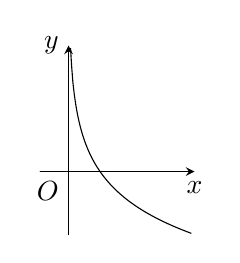
\begin{tikzpicture}[>=stealth,scale=.4, line join=round, line cap=round]
        \def\xmax{4} \def\ymin{-2} \def\ymax{4}
        %\draw[line width=0.1pt,dashed] (-0.9,\ymin) grid (\xmax,\ymax);
        \draw[->] (-0.9,0)--(\xmax,0) node [below]{$x$};
        \draw[->] (0,\ymin)--(0,\ymax) node [left]{$y$};
        \node at (0,0) [below left]{$O$};
        \clip (-0.9,\ymin) rectangle (\xmax-0.1,\ymax-0.1);
        \draw[smooth,samples=300,domain=0.03:\xmax] plot(\x,{ln(\x)/ln(0.5)});
    \end{tikzpicture}
}
%    \loigiai
%    {Quan sát hình dáng đồ thị ta thấy đồ thị nằm bên phải trục $Oy$, đồ thị đi xuống từ trái sang phải .
%    }
\end{ex}
%%==========Câu 2
\begin{ex}%[Lê Thị Thanh Tuyền-DA1]%[2D2B4-3]
\immini[thm]{
    Đường cong ở hình bên là của hàm số nào.
    \choice
    {$y=2^x$}
    {$y=\log_2 x$}
    {\True $y=\dfrac{1}{2^x}$}
    { $y=\log_{\frac{1}{2}} x$}
    
}{
    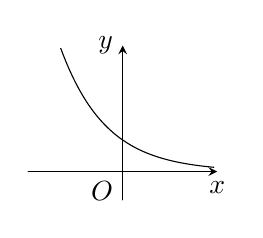
\begin{tikzpicture}[>=stealth,scale=.4, line join=round, line cap=round]
        \def\xmin{-3} \def\xmax{3} \def\ymax{4}
        %\draw[line width=0.1pt,dashed] (\xmin,-0.9) grid (\xmax,\ymax);
        \draw[->] (\xmin,0)--(\xmax,0) node [below]{$x$};
        \draw[->] (0,-0.9)--(0,\ymax) node [left]{$y$};
        \node at (0,0) [below left]{$O$};
        \clip (\xmin,-0.9) rectangle (\xmax-0.1,\ymax-0.1);
        \draw[smooth,samples=300] plot(\x,{0.5^(\x)});
    \end{tikzpicture}
}
%    \loigiai
%    {Quan sát hình dáng đồ thị ta thấy đồ thị nằm trên trục $Ox$, đồ thị đi xuống từ trái sang phải.
%    }
\end{ex}
%%==========Câu 3
%%==========Câu 4
\begin{ex}%[Lê Thị Thanh Tuyền-DA1]%[2D2B4-3]
\immini[thm] {
    Đường cong trong hình bên là đồ thị của hàm số nào.
    \choice
    {$y=e^x$}
    {\True $y=\log_{\sqrt{7}}x$}
    {$y=\log_{\frac{1}{2}} x$}
    {$y=\dfrac{1}{e^x}$}
}{
    \begin{tikzpicture}[>=stealth,scale=.4, line join=round, line cap=round]
        \def\xmax{4} \def\ymin{-2} \def\ymax{4}
        %\draw[line width=0.1pt,dashed] (-0.9,\ymin) grid (\xmax,\ymax);
        \draw[->] (-0.9,0)--(\xmax,0) node [below]{$x$};
        \draw[->] (0,\ymin)--(0,\ymax) node [left]{$y$};
        \node at (0,0) [below left]{$O$};
        \clip (-0.9,\ymin) rectangle (\xmax-0.1,\ymax-0.1);
        \draw[smooth,samples=300,domain=0.03:\xmax] plot(\x,{ln(\x)/ln(2.5)});
    \end{tikzpicture}
}
%    \loigiai{
%        Quan sát hình dáng đồ thị ta thấy đồ thị nằm bên phải trục $Oy$, đồ thị đi lên từ trái sang phải.
%    }
\end{ex}
\begin{ex}%[Lê Thị Thanh Tuyền-DA1][2D2B4-3]%
\immini[thm]
{
    Cho hai hàm số $y=\log_a x$ và $y=\log_b x$ có đồ thị như hình vẽ. Mệnh đề nào sau đây là đúng.
    \choice
    { $a>b>1$}
    {$1>a>b$}
    {\True$b>a>1$}
    {$a>1>b$}
}
{
    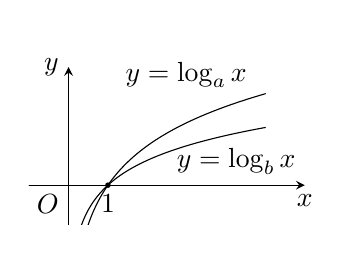
\begin{tikzpicture}[>=stealth,scale=.5, line join=round, line cap=round]
        \draw[->] (-1,0)--(6,0) node [below]{$x$};
        \draw[->] (0,-1)--(0,3) node [left]{$y$};
        \node at (0,0) [below left]{$O$};
        \node at (2.5,0.6)[right]{$y=\log_b x$};
        \node at (1.2,2.8)[right]{$y=\log_a x$};
        \clip (-1,-1) rectangle (6,4);
        \fill[black] (1,0) circle (2pt) node [below] {$1$};
        \draw[smooth,samples=150,domain=0.1:5] plot(\x,{ln(\x)/ln(3)});
        \draw[smooth,samples=150,domain=0.1:5] plot(\x,{ln(\x)/ln(2)});
    \end{tikzpicture}
}
\loigiai{
    \immini{
        Quan sát đồ thị ta thấy cả hai đồ thị đều đi lên từ trái sang phải nên $a>1$ và $b>1$.\\
        Kẻ đường thẳng $y=1$ lần lượt cắt hai đồ thị $y=\log_a x$ và $y=\log_b x$ tại hai điểm $A(a;1); B(b;1)$. \\Nhìn vào đồ thị ta thấy $a< b$.
    }
    {
        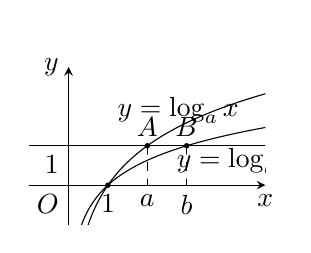
\begin{tikzpicture}[>=stealth,scale=.5, line join=round, line cap=round]
            \draw[->] (-1,0)--(5,0) node [below]{$x$};
            \draw[->] (0,-1)--(0,3) node [left]{$y$};
            \node at (0,0) [below left]{$O$};
            \clip (-1,-1) rectangle (5,4);
            \draw (-1,1)--(5,1) ;
            \fill[black] (1,0) circle (2pt) node [below] {$1$};
            \fill [black] (2,1) circle (2pt) node [above] {$A$};
            \fill [black] (3,1) circle (2pt) node [above] {$B$};
            \draw [dashed] (2,1)--(2,0) node [below] {$a$};
            \draw [dashed] (3,1)--(3,0) node [below] {$b$};
            \node at (0,1) [below left]{$1$};
            \draw[smooth,samples=150,domain=0.1:5] plot(\x,{ln(\x)/ln(3)});
            \draw[smooth,samples=150,domain=0.1:5] plot(\x,{ln(\x)/ln(2)});
            \node at (2.5,0.6)[right]{$y=\log_bx$};
            \node at (1,1.9)[right]{$y=\log_ax$};
        \end{tikzpicture}
    }
}
\end{ex}
%%==========Câu 9
\begin{ex}%[Lê Thị Thanh Tuyền-DA1][2D2K4-3]%
\immini[thm]{
    Cho các hàm số $y=a^x$; $y=\log_b x$ và $y=\log_c x$ có đồ thị như hình vẽ. Mệnh đề nào sau đây là đúng.
    \choice
    { \True $c>b>a$}
    {$b>a>c$}
    {$a>b>c$}
    {$b>c>a$}
}{
    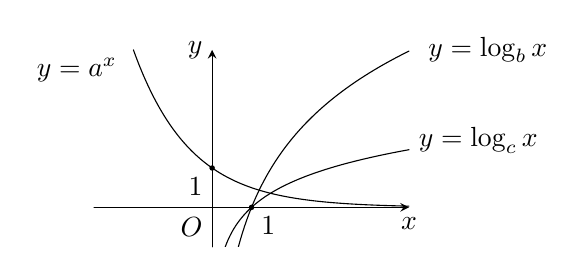
\begin{tikzpicture}[>=stealth,scale=.5, line join=round, line cap=round]
        \draw[->] (-3,0)--(5,0) node [below]{$x$};
        \draw[->] (0,-1)--(0,4) node [left]{$y$};
        \node at (0,0) [below left]{$O$};
        \node at (5,1.7)[right]{$y=\log_cx$};
        \node at (7,4){$y=\log_bx$};
        \node at (-4.7,3.5)[right]{$y=a^x$};
        \clip (-3,-1) rectangle (7,4);
        \fill[black] (1,0) circle (2pt) node [below right] {$1$} (0,1) circle (2pt) node [below left] {$1$};
        \draw[smooth,samples=150,domain=0.1:5] plot(\x,{ln(\x)/ln(3)});
        \draw[smooth,samples=150,domain=0.1:5] plot(\x,{ln(\x)/ln(1.5)});
        \draw[smooth,samples=150,domain=-2:5] plot(\x,{2^(-\x)});
    \end{tikzpicture}
}
%    \loigiai{
%        Quan sát đồ thị ta thấy
%        \begin{itemize}
%            \item Cả hai đồ thị của hàm số $y=\log_b x$ và $y=\log_c x$ đều đi lên từ trái sang phải nên $b>1$ và $c>1$.
%            \item Đồ thị của hàm số $y=a^x$ đi xuống từ trái sang phải nên $0<a<1$.
%            \item Kẻ đường thẳng $y=1$ lần lượt cắt hai đồ thị $y=\log_b x$ và $y=\log_c x$ tại hai điểm $A(b;1); B(c;1)$. Nhìn vào đồ thị ta thấy $b< c$.\\
%            Vậy $a<b<c$.
%        \end{itemize}
%    }
\end{ex}
\begin{ex}%[2D2Y5-1]
Nghiệm của phương trình $3^{x-1}=27$ là
\choice
{\True $x=4$}
{$x=3$}
{$x=2$}
{$x=1$}
\loigiai{
    Ta có\\
    $3^{x-1}=27\Leftrightarrow x-1=3\Leftrightarrow x=4$.
}
\end{ex}
%Câu 41
\begin{ex}
Phương trình $7^x=5$ có nghiệm là
\choice
{$\log_57$}
{$-\log_57$}
{$-\log_75$}
{\True $\log_75$}
%    \loigiai{
%        Ta có $7^x=5 \Leftrightarrow x=\log_75$.
%    }
\end{ex}
\begin{ex}%[Đề minh họa 2023]%[2D2B6-2]
Tập nghiệm của bất phương trình $2^{x+1}<4$ là
\choice
{$(-\infty;1]$}
{$(1;+\infty)$}
{$[1;+\infty)$}
{\True $(-\infty;1)$}
\loigiai{
    \[2^{x+1}<4 \Leftrightarrow 2^{x+1}<2^2 \Leftrightarrow x+1<2\Leftrightarrow x<1.\]
    Vậy tập nghiệm của bất phương trình là $(-\infty;1)$.
}
\end{ex}
\begin{ex}%[Đề minh họa 2023]%[2D2Y6-1]
Tập nghiệm của bất phương trình $\log (x-2)>0$ là
\choice
{$(2;3)$}
{$(-\infty;3)$}
{\True $(3;+\infty)$}
{$(12;+\infty)$}
\loigiai{
    Điều kiện $x-2>0\Leftrightarrow x>2$.\\
    Ta có $\log (x-2)>0\Leftrightarrow x-2>1\Leftrightarrow x>3$.\\
    Kết hợp điều kiện ta có tập nghiệm $(3;+\infty)$.
}
\end{ex}
\begin{ex}%[Mã đề 101 - 2022]%[2D2Y5-1]
Tập nghiệm của bất phương trình $ \log _5(x+1)>2 $ là
\choice
{$ (9;+\infty) $}
{$ (25;+\infty) $}
{$ (31;+\infty) $}
{\True $ (24;+\infty) $}
\loigiai{
    Ta có $ \log _5(x+1)>2\Leftrightarrow x+1>5^2\Leftrightarrow x+1>25\Leftrightarrow x>24 $. \\
    Vậy tập nghiệm của bất phương trình là $ (24;+\infty) $.
}
\end{ex}
\begin{ex}%[2D2B6-1]
Tập nghiệm của bất phương trình $\log_{\frac{\pi}{6}}\left[\log_3\left(x-2\right)\right]>0$ là khoảng $\left(a;b\right)$. Giá trị $b-a$ bằng
\choice
{\True $2$}
{$4$}
{$3$}
{$5$}
\loigiai{
    Ta có $0<\dfrac{\pi}{6}<1$ nên\\
    $\log_{\frac{\pi}{6}}\left[ \log_3\left(x-2\right)\right]>0 \Leftrightarrow 0<\log_3\left(x-2\right)<1 \Leftrightarrow 1<x-2<3 \Leftrightarrow 3<x<5$.\\
    Do đó, $a=3$ và $b=5$.\\
    Vậy $b-a=2$.
}
\dotlineEX{2}% Tạo các dòng kẻ trong tài liệu
\end{ex}
\begin{ex}%[1D6H4-2]
Cho hàm số $f(x)=\left(\dfrac{1}{3} \right)^x$.
\choiceTF
{Tập xác định của hàm số $f(x)$ là $\mathscr{D}=(0;+\infty)$}
{\True Phương trình $f(x)=m$ có nghiệm khi và chỉ khi $m > 0$}
{\True $f(-2)=9$}
{Tập nghiệm của phương trình $f(x) = 27^{x^2}$ là $S=\left\{-1;-\dfrac{1}{3} \right\}$}
\loigiai{
    \begin{itemchoice}
        \itemch {\bf Sai}.\\ Tập xác định $\mathscr{D}=\mathbb{R}$.
        \itemch {\bf Đúng}. \\
        Xét phương trình $\left(\dfrac{1}{3} \right)^x=m$.\\
        Vì $\left(\dfrac{1}{3} \right)^x>0$, $\forall x \in \mathbb{R}$ nên phương trình có nghiệm khi và chỉ khi $m>0$.
        \itemch {\bf Đúng}.\\ Ta có $f(-2)=\left(\dfrac{1}{3} \right)^{-2}=3^2=9$.
        \itemch {\bf Sai}.\\
        Ta có
        \begin{eqnarray*}
            & &f(x) > 27^{x^2}\\
            &\Leftrightarrow& \left(\dfrac{1}{3} \right)^x= 27^{x^2}\\
            &\Leftrightarrow& (3)^{-x}=(3^3)^{x^2}\\
            &\Leftrightarrow& -x=3x^2\\
            &\Leftrightarrow& \hoac{& x=0\\& x=-\dfrac{1}{3}.}
        \end{eqnarray*}
        Vậy $S=\left\{-\dfrac{1}{3};0 \right\}$.
    \end{itemchoice}	
}
\dotlineEX{2}% Tạo các dòng kẻ trong tài liệu
\end{ex}
\begin{ex}%[1D6V4-2]
Cho hàm số $y=\log_3\left(x^2-x-2\right)$.
\choiceTF
{Tập xác định $\mathscr{D}$ của hàm số là $\mathscr{D}=(-\infty;-1]\cup[2;+\infty)$}
{\True Phương trình $\log_3\left(x^2-x-2\right)=\log_3(4x-2)$ có duy nhất một nghiệm}
{\True $y'(3)>0$}
{Giá trị lớn nhất của hàm số $y=\log_3\left(x^2-x-2\right)$ trên đoạn $[\mathrm{e};3]$ là $4$}
\loigiai{
    \begin{itemchoice}
        \itemch \textbf{Sai.} \\
        Hàm số xác định khi $x^2-x-2>0\Leftrightarrow\hoac{&x<-1\\&x>2.}$\\
        Tập xác định của hàm số là $\mathscr{D}=(-\infty;-1)\cup(2;+\infty)$.
        \itemch \textbf{Đúng.} \\
        Ta có
        $$\log_3\left(x^2-x-2\right)=\log_3(4x-2)\Leftrightarrow\heva{&4x-2>0\\&x^2-x-2=4x-2}\Leftrightarrow\heva{&x>\dfrac{1}{2}\\&x^2-5x=0}\Leftrightarrow x=5.$$
        Vậy phương trình có duy nhất một nghiệm nguyên.
        \itemch \textbf{Đúng.} \\
        Ta có $y'=\dfrac{2x-1}{\left(x^2-x-2\right)\ln3}$ nên $y'(3)=\dfrac{5}{4\ln{3}}>0$.
        \itemch \textbf{Sai.} \\
        Vì $y'=0\Leftrightarrow x=\dfrac{1}{2} \notin [\mathrm{e};3]$ và $y'>0$ với $x>2$ nên giá trị lớn nhất của hàm số trên đoạn $[\mathrm{e};3]$ là $y(3)=\log_34$.
    \end{itemchoice}
}
\dotlineEX{6}% Tạo các dòng kẻ trong tài liệu
\end{ex}
\begin{ex}%[1D6V4-4]
Cho phương trình $\log (x-1)^2=\log (x+1)$. Khi đó
\choiceTF
{Điều kiện $x > 1$}
{Phương trình đã cho có chung tập nghiệm với phương trình $x^2-3x+\dfrac{9}{4}=0$}
{\True Tổng các nghiệm của phương trình bằng $3$}
{\True Biết phương trình có hai nghiệm $x_1, x_2 \left(x_1 < x_2 \right)$. Khi đó 3 số $x_1;x_2;6$ tạo thành một cấp số cộng}
\loigiai{
    Điều kiện $\heva{&{(x-1)^2> 0} \\
        &{x+1> 0}.}$(*)
    \[\log (x-1)^2=\log (x+1)\Rightarrow (x-1)^2=x+1\Leftrightarrow x^2-3x=0\Leftrightarrow \hoac{&{x=0} \\
        &{x=3}}
    \]
    Thay lần lượt hai giá trị này vào $(*)$, ta thấy cả hai giá trị đều thoả mãn. Vậy phương trình có tập nghiệm là $S=\{0;3\}$.
    \begin{itemchoice}
        \itemch Sai
        \itemch Sai. Vì $x=0$ không có nghiệm $x^2-3x+\dfrac{9}{4}=0$.
        \itemch Đúng. Vì Tổng các nghiệm của phương trình bằng $0+3=3$.
        \itemch Đúng. Vì $0;3;6$ tạo thành một cấp số cộng
    \end{itemchoice}	
}
  \dotlineEX{2}% Tạo các dòng kẻ trong tài liệu
\end{ex}

\begin{ex}%[1D6H4-3]%[Chủ đề: Bất phương trình mũ và bất phương trình logarit - Dự án C đợt 2 - năm học 2024 - 2025 - Nguyễn Hoàng Anh]
Cho bất phương trình $\left(\dfrac{1}{3}\right)^{2x^2-3x-7}>3^{2x-21}$ là
\choiceTF
{\True $\left(\dfrac{1}{3}\right)^{2x^2-3x-7}=3^{-2x^2+3x+7}$}
{\True Bất phương trình đã cho tương đương với bất phương trình $-2x^2+x+28>0$}
{\True Tập nghiệm của bất phương trình đã cho là $\left(-\dfrac{7}{2}; 4\right)$}
{Bất phương trình có $6$ nghiệm nguyên}
\loigiai{
    \begin{itemchoice}
        \itemch \textbf{Đúng}. Vì $\left(\dfrac{1}{3}\right)^{2x^2-3x-7}=\left[(3)^{-1}\right]^{2x^2-3x-7}=3^{-2x^2+3x+7}$.
        \itemch \textbf{Đúng}. Vì
        \begin{eqnarray*}
            &&\left(\dfrac{1}{3}\right)^{2x^2-3x-7}>3^{2x-21}\\
            &\Leftrightarrow&{3^{-(2x^2-3x-7)}}>3^{2x-21}\\
            &\Leftrightarrow& -(2x^2-3x-7)>2x-21\\
            &\Leftrightarrow &-2x^2+3x+7>2x-21\\
            &\Leftrightarrow& -2x^2+x+28>0.
        \end{eqnarray*}
        \itemch \textbf{Đúng}. Vì $-2x^2+x+28>0 \Leftrightarrow -\dfrac{7}{2}<x<4$.
        Do đó tập nghiệm của bất phương trình đã cho là $\left(-\dfrac{7}{2}; 4\right)$.
        \itemch \textbf{Sai}. Vì có $7$ số nguyên thuộc khoảng $\left(-\dfrac{7}{2}; 4\right)$ là $\left\{-3;-2;-1;0;1;2;3\right\}$.
    \end{itemchoice}
}
\dotlineEX{4}% Tạo các dòng kẻ trong tài liệu
\end{ex}
\begin{ex}
\immini[thm]{ Đồ thị các hàm số $y = \log_a x$, $y = \log_b x$, $ y = \log_c x$ được cho trong hình vẽ bên.
    \choiceTF
    {\True Có đúng hai hàm số đã cho đồng biến trên các tập xác định của nó}
    {\True $\log_c x > \log_c 2 \Rightarrow x < 2$}
    { $c < b < a$}
    {Đường thẳng $y = 3$ cắt trục $Oy$ và cắt đồ thị các hàm số $y = \log_a x, y = \log_b x$ lần lượt tại các điểm $M, N, P$ sao cho $N$ là trung điểm của $MP$. Khi đó $a^3 = 2b^3$}
}{
    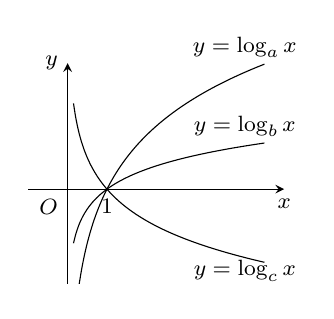
\begin{tikzpicture}[font=\footnotesize, >=stealth, yscale=0.4,xscale=.5]
        \draw[->] (-1,0) -- (5.5,0) node[below] {$x$};
        \draw[->] (0,-3) -- (0,4) node[left] {$y$};
        \node at (0,0) [below left] {$O$};
        \fill (1,0) circle (1.2pt) node[below] {$1$};
        \node at (4.5,4.5) {$y=\log_a x$};
        \node at (4.5,2) {$y=\log_b x$};
        \node at (4.5, -2.6) {$y=\log_c x$};
        \clip (-1,-3) rectangle (6,4.3);
        \draw[smooth, samples=100, domain=0.2:5] plot(\x, {ln(\x)/ln(1.5)});
        \draw[smooth, samples=100, domain=0.15:5] plot(\x, {ln(\x)/ln(3)});
        \draw[smooth, samples=100, domain=0.15:5] plot(\x, {-ln(\x)/ln(2)});
    \end{tikzpicture}
}
\loigiai{
    \begin{itemize}
        \item \textbf{Ý a) Đúng:} Quan sát đồ thị ta thấy hàm số $y = \log_a x$ và $y = \log_b x$ có đồ thị đi lên từ trái sang phải nên là các hàm số đồng biến $\Rightarrow a > 1, b > 1$. Hàm số $y = \log_c x$ có đồ thị đi xuống nên là hàm số nghịch biến $\Rightarrow 0 < c < 1$. Vậy có đúng hai hàm số đồng biến.
        \item \textbf{Ý b) Đúng:} Do $0 < c < 1$ nên hàm số $y = \log_c x$ nghịch biến trên khoảng $(0; +\infty)$. 
        Khi đó $\log_c x > \log_c 2 \Leftrightarrow 0 < x < 2$. Do đó mệnh đề $\Rightarrow x < 2$ là đúng.
        \item \textbf{Ý c) Sai:} Kẻ đường thẳng $y = 1$ cắt đồ thị $y = \log_a x$ tại điểm có hoành độ $x = a$ và cắt đồ thị $y = \log_b x$ tại điểm có hoành độ $x = b$. Dựa vào đồ thị, ta thấy $1 < a < b$. Kết hợp với $0 < c < 1$, ta có thứ tự đúng là $c < a < b$.
        \item \textbf{Ý d) Sai:} Giao điểm của đường thẳng $y = 3$ với trục $Oy$ là $M(0; 3)$.
        Giao điểm của $y = 3$ với đồ thị $y = \log_a x$ là nghiệm của phương trình $\log_a x = 3 \Leftrightarrow x = a^3 \Rightarrow N(a^3; 3)$.
        Giao điểm của $y = 3$ với đồ thị $y = \log_b x$ là nghiệm của phương trình $\log_b x = 3 \Leftrightarrow x = b^3 \Rightarrow P(b^3; 3)$.
        Vì $N$ là trung điểm của đoạn thẳng $MP$ nên ta có:
        $$x_N - x_M = x_P - x_N \Leftrightarrow a^3 - 0 = b^3 - a^3 \Leftrightarrow 2a^3 = b^3$$
        Phát biểu cho rằng $a^3 = 2b^3$ là sai.
    \end{itemize}
}
\dotlineEX{3}% Tạo các dòng kẻ trong tài liệu
\end{ex}
\begin{ex}
\immini[thm]{ Cho các hàm số $y = 2^{x+1}$ và $y = 2^{3-x}$ có đồ thị như hình vẽ bên.
    \choiceTF
    {\True Đồ thị hàm số $y = 2^{x+1}$ cắt trục tung tại điểm $A(0; 2)$}
    { Đồ thị hàm số $y = 2^{3-x}$ cắt trục tung tại điểm $B(0; 6)$}
    { Giao điểm $C$ của hai đồ thị có hoành độ bằng $1$}
    { Diện tích tam giác $ABC$ bằng $6$}
}{
    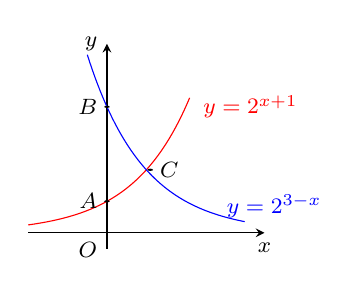
\begin{tikzpicture}[>=stealth, yscale=0.2,xscale=.5, font=\footnotesize]
        \draw[->] (-2,0) -- (4,0) node[below] {$x$};
        \draw[->] (0,-1) -- (0,12) node[left] {$y$};
        \node at (0,0) [below left] {$O$};
        \draw[red, smooth, samples=100, domain=-2:2.1] plot(\x, {2^(\x+1)});
        \draw[blue, smooth, samples=100, domain=-0.5:3.5] plot(\x, {2^(3-\x)});
        \fill (0,2) circle (2pt) node[left] {$A$};
        \fill (0,8) circle (2pt) node[left] {$B$};
        \fill (1.1,4) circle (2pt) node[right] {$C$};
        \node[red] at (2.2, 8) [right] {$y=2^{x+1}$};
        \node[blue] at (2.8, 1.7) [right] {$y=2^{3-x}$};
    \end{tikzpicture}
}
\loigiai{
    \begin{itemize}
        \item \textbf{Ý a) Đúng:} Điểm $A$ là giao điểm của đồ thị hàm số $y = 2^{x+1}$ với trục tung ($x=0$). 
        Thay $x=0$ vào hàm số, ta được $y = 2^{0+1} = 2$. Vậy $A(0; 2)$.
        \item \textbf{Ý b) Sai:} Điểm $B$ là giao điểm của đồ thị hàm số $y = 2^{3-x}$ với trục tung ($x=0$).
        Thay $x=0$ vào hàm số, ta được $y = 2^{3-0} = 2^3 = 8$. Vậy $B(0; 8)$. 
        \textit{(Phát biểu cho tung độ bằng $6$ là một bẫy sai lầm phổ biến khi học sinh tính nhầm $2 \cdot 3 = 6$ thay vì lũy thừa $2^3 = 8$)}.
        \item \textbf{Ý c) Đúng:} Điểm $C$ là giao điểm của hai đồ thị. Hoành độ của $C$ là nghiệm của phương trình:
        $$2^{x+1} = 2^{3-x}$$
        $$\Leftrightarrow x + 1 = 3 - x$$
        $$\Leftrightarrow 2x = 2 \Leftrightarrow x = 1$$
        Vậy hoành độ của điểm $C$ là $x = 1$. (Thay vào hàm số ta tính được tung độ $y = 2^{1+1} = 4$, suy ra $C(1; 4)$).
        \item \textbf{Ý d) Sai:} Ta có $A(0; 2)$ và $B(0; 8)$ cùng nằm trên trục $Oy$ nên độ dài cạnh đáy $AB$ là khoảng cách giữa hai tung độ:
        $$AB = |y_B - y_A| = |8 - 2| = 6$$
        Đường cao $h$ hạ từ đỉnh $C(1; 4)$ xuống trục $Oy$ chính là giá trị tuyệt đối hoành độ của $C$, tức là $h = |x_C| = 1$.
        Diện tích tam giác $ABC$ là:
        $$S = \frac{1}{2} \cdot AB \cdot h = \frac{1}{2} \cdot 6 \cdot 1 = 3$$
        \textit{(Phát biểu cho kết quả bằng $6$ để bẫy những học sinh quên nhân hệ số $\frac{1}{2}$ trong công thức tính diện tích tam giác).}
    \end{itemize}
}
\dotlineEX{1}% Tạo các dòng kẻ trong tài liệu
\end{ex}
\begin{ex}%[1D6V4-6]%[GV:Xuan Vy Pham]
Một nhóm các chuyên gia y tế đang nghiên cứu và thử nghiệm độ chính xác của một xét nghiệm COVID-19. Giả sử cứ sau $n$ lần thử nghiệm và điều chỉnh thì tỉ lệ chính xác của bộ xét nghiệm đó tuân theo công thức $S(n)=\dfrac{1}{1+2020 \cdot 10^{-0{,}01n}}$. Hỏi phải tiến hành ít nhất bao nhiêu lần thử nghiệm và điều chỉnh bộ xét nghiệm để đảm bảo độ chính xác của bộ xét nghiệm đo trên $90\%$?
\shortans{}
\loigiai
{Để đảm bảo độ chính xác của bộ xét nghiệm đo trên $90\%$ thì số lần thử nghiệm $n$ thỏa
    \allowdisplaybreaks
    \begin{align*}
        S(n)>90\% &\Leftrightarrow\dfrac{1}{1+2020 \cdot 10^{-0{,}01n}}>90\%\\
        &\Leftrightarrow 1+2020 \cdot 10^{-0{,}01n} < \dfrac{100}{90}\\
        &\Leftrightarrow 2020 \cdot 10^{-0{,}01n} <\dfrac{1}{9}\\
        &\Leftrightarrow 10^{-0{,}01n}<\dfrac{1}{18180}\\
        &\Leftrightarrow -0{,}01n< \log \dfrac{1}{18180}\\
        &\Leftrightarrow n> -\dfrac{1}{0{,}01}\log \dfrac{1}{18180}.
    \end{align*}
    Số tự nhiên $n$ nhỏ nhất thỏa $n> -\dfrac{1}{0{,}01}\log \dfrac{1}{18180}$ là $426$.\\
    Vậy phải tiến hành ít nhất $426$ lần thử nghiệm và điều chỉnh bộ xét nghiệm để đảm bảo độ chính xác của bộ xét nghiệm đo trên $90\%$.
}
\dotlineEX{1}% Tạo các dòng kẻ trong tài liệu
\end{ex}
\begin{ex}%[1D6C4-6]
Dân số thế giới được ước tính theo công thức $S=A \cdot \mathrm{e}^{rN}$, trong đó: $A$ là dân số của năm lấy mốc tính, $S$ là dân số sau $N$ năm, $r$ là tỉ lệ tăng dân số hằng năm. Ngày $15/11/2022$, dân số thế giới khoảng $8$ tỉ người. Cho biết $r=1{,}32 \%$, hãy cho biết ngày $15 / 11 / 2032$ dân số thế giới khoảng bao nhiêu tỉ người (làm tròn kết quả đến hàng phần trăm).
\shortans{$7{,}01$}
\loigiai{
    Từ $15/11/2022$ đến $15/11/2032$ là $10$ năm. Suy ra $N=10$.\\
    Theo đề ra, ta có
    \begin{eqnarray*}
        S=A \cdot \mathrm{e}^{rN}=8 \Rightarrow A=\dfrac{8}{\mathrm{e}^{rN}} \approx 7{,}01 \text{ tỉ dân.}
    \end{eqnarray*}
}
  \dotlineEX{6}% Tạo các dòng kẻ trong tài liệu
\end{ex}
\begin{ex}%[1D6V4-5] 
Các khí thải gây hiệu ứng nhà kính là nguyên nhân chủ yếu làm Trái đất nóng lên. Theo OECD (Tổ chức Hợp tác và Phát triển kinh tế thế giới), khi nhiệt độ Trái đất tăng lên thì tổng giá trị kinh tế toàn cầu giảm. Người ta ước tính rằng, khi nhiệt độ Trái đất tăng thêm $2^{\circ} \mathrm{C}$ thì tổng giá trị kinh tế toàn cầu giảm $3 \%$; còn khi nhiệt độ Trái đất tăng thêm $5^{\circ} \mathrm{C}$ thì tổng giá trị kinh tế toàn cầu giảm $10 \%$. Biết rằng, nếu nhiệt độ Trái đất tăng thêm $t^{\circ} \mathrm{C}$, tổng giá trị kinh tế toàn cầu giảm $f(t) \%$ thì $f(t)=k \cdot a^t$ trong đó $k$, $a$ là các hằng số dương. Khi nhiệt độ Trái đất tăng thêm bao nhiêu độ thì tổng giá trị kinh tế toàn cầu giảm đến $25\%$ (kết quả làm tròn đến hàng phần chục)?
\shortans{$7{,}3$}
\loigiai{
    Ta có $\heva{k\cdot a^2=3 \% \\ k \cdot a^5=10 \%} \Rightarrow a=\sqrt[3]{\dfrac{10}{3}} ; k=\dfrac{3 \%}{a^2}$.\\
    Tổng giá trị kinh tế toàn cầu giảm đến $25 \%$ nên ta có $$\dfrac{3 \%}{a^2} \cdot a^t=25 \% \Rightarrow a^{t-2}=\dfrac{25}{3}\Rightarrow t=2+\log _a \dfrac{25}{3}=2+\log _{\sqrt{\frac{10}{3}}} \dfrac{25}{3} \approx 7,3.$$
}
  \dotlineEX{3}% Tạo các dòng kẻ trong tài liệu
\end{ex}
\begin{ex}%[1D6V4-5] 
Theo một bài báo được công bố trên tạp chí Nature, trung bình làm cha ở tuổi $30$ sẽ có $55$ đột biến cho con cái của mình. Đột biến này tăng theo độ tuổi. Cứ tăng $1$ tuổi, số lượng đột biến sẽ tăng thêm $12 \%$ so với số lượng đột biến trước đó. Hỏi sau ít nhất bao nhiêu năm thì số lượng đột biến đạt đến $15800$.
\shortans{$50$}
\loigiai{
    Gọi $A_0$ là số lượng đột biến mà trung bình làm cha ở tuổi $30$ gây ra cho con cái của mình $\Rightarrow A_0=55$ đột biến.
    Gọi $r$ là tốc độ tăng đột biến $\Rightarrow r=12 \%$.\\
    Sau $n$ năm só lượng đột biến là $A=A_0(1+r)^n$.\\
    Ta có $15800=55(1+12 \%)^n \Rightarrow n=\log _{1,12} \dfrac{15800}{55} \approx 49,95$.\\
    Vậy sau ít nhất $50$ năm thì số lượng đột biến đạt đến $15800$.	
}
\dotlineEX{4}% Tạo các dòng kẻ trong tài liệu
\end{ex}
\begin{ex}%[1D6V4-5] 
Để ước tính dân số người ta sử dụng công thức $A_{\mathrm{N}}=A \mathrm{e}^{\mathrm{rN}}$, trong đó $A$ là dân số của năm lấy làm mốc tính, $A_N$ là dân số sau $N$ năm, $r$ là tỉ lệ tăng dân số hàng năm. Biết rằng dân số Việt Nam ở các năm $2014$ và $2024$ lần lượt là $85{,}9$ và $96{,}2$ triệu người. Hỏi ở năm nào dân số nước ta sẽ vượt qua ngưỡng $120$ triệu người ?
\shortans{$2044$}
\loigiai{
    Giả sử năm $2014$ là năm lấy làm mốc tính $k$ năm.\\
    Nên dân số năm $2014$ là $A_k=A \mathrm{e}^{r k}=85{,}9$ (triệu người).\\
    Suy ra tại năm $(2014+m),(m \in \mathbb{Z})$ dân số sẽ là
    $A_{k+m}=A \mathrm{e}^{r(k+m)}=A \mathrm{e}^{r k} \cdot \mathrm{e}^{m m}=85{,}9 \cdot \mathrm{e}^{m m}$ (triệu người).\\
    Như vậy dân số năm $2024$ là $85{,}9 . \mathrm{e}^{10 r}=96{,}2$ (triệu người).
    $$
    \Rightarrow \mathrm{e}^{10 r}=\frac{96{,}2}{85{,}9} \Rightarrow \mathrm{e}^r=\sqrt[10]{\frac{962}{859}} .
    $$
    Theo bài toán ta có $$85,9 \cdot \mathrm{e}^{r m}>120 \Rightarrow m>\log _{\mathrm{e}^r} \frac{96{,}2}{85{,}9}\left(\right. \text{do} \left.\mathrm{e}^r>1\right) \Rightarrow m>29{,}52 \Rightarrow m \geq 30.$$
    Như vậy tại năm $2044$, dân số sẽ vượt ngưỡng $120$ triệu người.	
}
   \dotlineEX{4}% Tạo các dòng kẻ trong tài liệu
\end{ex}
\begin{ex}
Trên mỗi chiếc radio đều có các vạch chia để người sử dụng dễ dàng chọn đúng sóng radio cần tìm. Biết rằng vạch chia ở vị trí cách vạch tận cùng bên trái một khoảng $d$ (cm) thì ứng với tần số $F = k \cdot a^d$ (kHz), trong đó $k$ và $a$ là hai hằng số được chọn sao cho vạch tận cùng bên trái ứng với tần số $620 \text{ kHz}$, vạch tận cùng bên phải ứng với tần số $1710 \text{ kHz}$ và hai vạch này cách nhau $20 \text{ cm}$. Hỏi vạch chia ứng với tần số $1000 \text{ kHz}$ nằm cách vạch tận cùng bên trái một khoảng bao nhiêu xentimét? \textit{(Làm tròn kết quả đến hàng phần mười)}.
\shortans{$9{,}4$}
\loigiai{
    Chọn mốc khoảng cách $d=0$ tại vạch tận cùng bên trái. Khi đó:
    \begin{itemize}
        \item Tại vạch tận cùng bên trái ($d = 0$), tần số $F(0) = 620 \text{ kHz}$.
        Thay vào công thức ta được: $k \cdot a^0 = 620 \Rightarrow k = 620$.
        \item Tại vạch tận cùng bên phải ($d = 20 \text{ cm}$), tần số $F(20) = 1710 \text{ kHz}$.
        Thay $k=620$ và $d=20$ vào công thức, ta có:
        $$620 \cdot a^{20} = 1710 \Leftrightarrow a^{20} = \frac{1710}{620} = \frac{171}{62} \Rightarrow a = \left(\frac{171}{62}\right)^{\frac{1}{20}}$$
    \end{itemize}
    Để tìm vị trí vạch chia ứng với tần số $1000 \text{ kHz}$, ta cần tìm $d$ thỏa mãn $F(d) = 1000$:
    $$620 \cdot a^d = 1000 \Leftrightarrow a^d = \frac{100}{62} = \frac{50}{31}$$
    Lấy logarit cơ số $a$ hai vế, ta được:
    $$d = \log_a \left(\frac{50}{31}\right) = \frac{\ln\left(\frac{50}{31}\right)}{\ln a} = \frac{\ln\left(\frac{50}{31}\right)}{\ln\left[\left(\frac{171}{62}\right)^{\frac{1}{20}}\right]} = \frac{\ln\left(\frac{50}{31}\right)}{\frac{1}{20}\ln\left(\frac{171}{62}\right)}$$
    $$d = 20 \cdot \frac{\ln\left(\frac{50}{31}\right)}{\ln\left(\frac{171}{62}\right)} \approx 9{,}428 \text{ (cm)}$$
    Làm tròn kết quả đến hàng phần mười, ta được $d \approx 9{,}4 \text{ cm}$.
    \textbf{Đáp án:} $9{,}4$
}
   \dotlineEX{4}% Tạo các dòng kẻ trong tài liệu
\end{ex}
\Closesolutionfile{ans}